Секция содержит постановки научных работ на текущий момент находящиеся в исследовании. 

\begin{figure}[h]
    \centering
    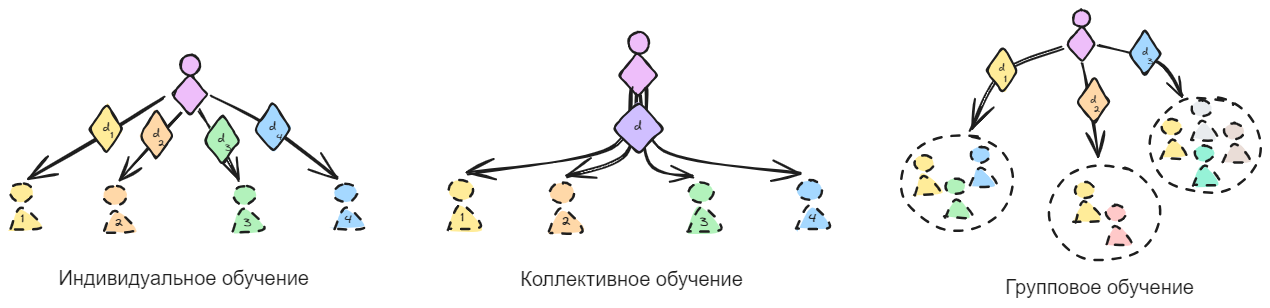
\includegraphics[width=0.5\textwidth]{assets/final/setting.excalidraw.png}
    \caption{Групповое обучение позволяет задать баланс между объемом проверки и специфичностью задания}
    \label{group_learning}
\end{figure}

Совместное обучение подразумевает одновременное достижение высоких уровней компетенций в предмете изучения.
Такое обучения, как правило, сопровождается подготовленным методическими материалами общими для всех обучающихся.
Задача преподавателя в наиболее успешном прохождение учащихся методической программы. При внесении изменений
в курс оценивается изменение среднего показателя учащихся. Усредненные аналитические показатели позволяют принимать решения с статически заданными
порогами риска и приобретений. Это обеспечивает устойчивые рост образования в среднем. Для развития практики
полезно учитывать индивидуальные потребности учащихся, заключающиеся в разном уровне освоения материала и задачах его использования. Разрешить проблему
можно путем индивидуального образования, но такой подход осложнен увеличением преподавательской нагрузки. Одним из компромиссных решений является групповое образование,
обеспечивающее баланс между специфичностью задания для учащегося и временем для проверки для преподавателя.

Обучение в группах требует аналитического описания в трех направлениях: \begin{enumerate}
    \item определение правил объединения в группы
    \item подбор сложности задания для группы, включающий модель оценки эффективности совместной работы
    \item оценка распределения нагрузки в случае группового задания
\end{enumerate}

Разработанный в работе алгоритм адаптивного подбор сложности применим только в постановках индивидуального обучения, практическое применение которого
актуально для цифровых систем. В постановке коллективного обучения предложенный алгоритм сможет обеспечить оптимальный уровень сложности для всего коллектива в общем.
Такая модель слишком груба,поскольку не учитывается важные для образовательного коллектива процессы соревнования и кооперации учащихся. Учет коллективных эффектов
выполняется в постановках распределенной оптимизации, теории марковских полей и теоретической физике. Для анализа малых групп используются 
ковариационные матрицы и супераддитивные функции. 

Супераддитивной называется функция $f$ для которой
\begin{equation}
    \forall x, y, x+y \in \text{dom}(f) \rightarrow f(x+y) \ge f(x) +f(y) 
\end{equation}

Такие функции позволяю оценить по индивидуальным качествам учащихся их совместный вклад в дело. Примерами супераддитивных функций являются \begin{itemize}
    \item min-sum $\sum_{i} min([\vec{x}]_i,s^*)$, гдe $s^*$ - порог отсечки
    \item max-mean $N \cdot \bar{x} + \max_i(\vec{x} - \bar{x})$
    \item квадратичная форма $\vec{x}^T A \vec{x}$
\end{itemize}

\begin{figure}[h]
    \centering
    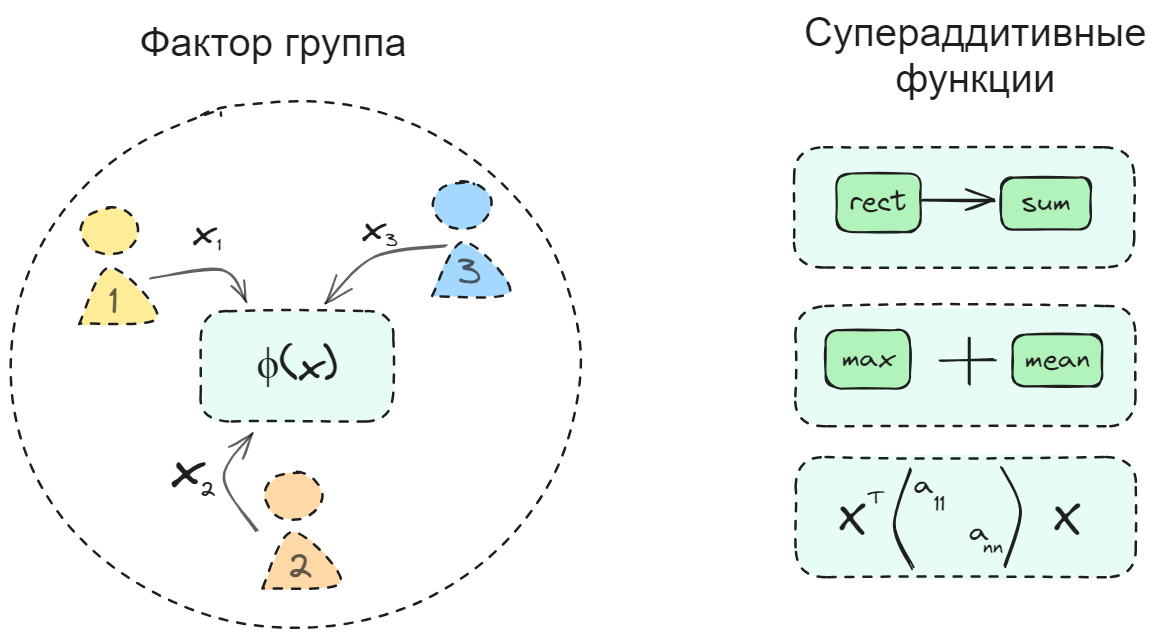
\includegraphics[width=0.5\textwidth]{assets/final/group.excalidraw.png}
    \caption{Uрупповые задания}
    \label{group_task}
\end{figure}



Практически функцию улучшение среднего результата в классе. 

Общий результат лучше исключает
случайности и может быть оценкой эффективности как отдельного педагога, так и всего преподавательского коллектива.
Тем не менее такой подход не всегда может учесть индивидуальные образовательные потребности учащихся. Одним из возможных
разрешений такой проблемы является объединение учащихся в группы для выполнения задач.




Также автор отмечает высокий потенциал направления символьной регрессии,
использованный в известной работы команды DeepMind \cite{trinh2024solving}. Принципиальнj
методика решения заключается в использовании
Предложенный метод имеет подтвержденную эффективность, реализация алгоритма позволяет решает
задачи из международной олимпиады по математике с рейтингом на уровне победителей.












